From equations (4.22) one might be tempted to try to implement SOR as
\begin{verbatim}
     for iter=1:maxiter
        uGS = (DA - LA) \ (UA*u + rhs);
        u = u + omega * (uGS - u);
     end
\end{verbatim}

where the matrices have been defined as in \verb+iter_bvp_Asplit.m+. Try this computationally and observe that it does
not work well. Explain what is wrong with this and derive the correct expression (4.24).

\begin{solution}\ \\\\
    We implement the above SOR algorithm as the \texttt{naive\_SOR} case in \texttt{problem\_1d.m}. The corresponding
    error plot is shown below:

    \begin{figure}[h]
        \centering
        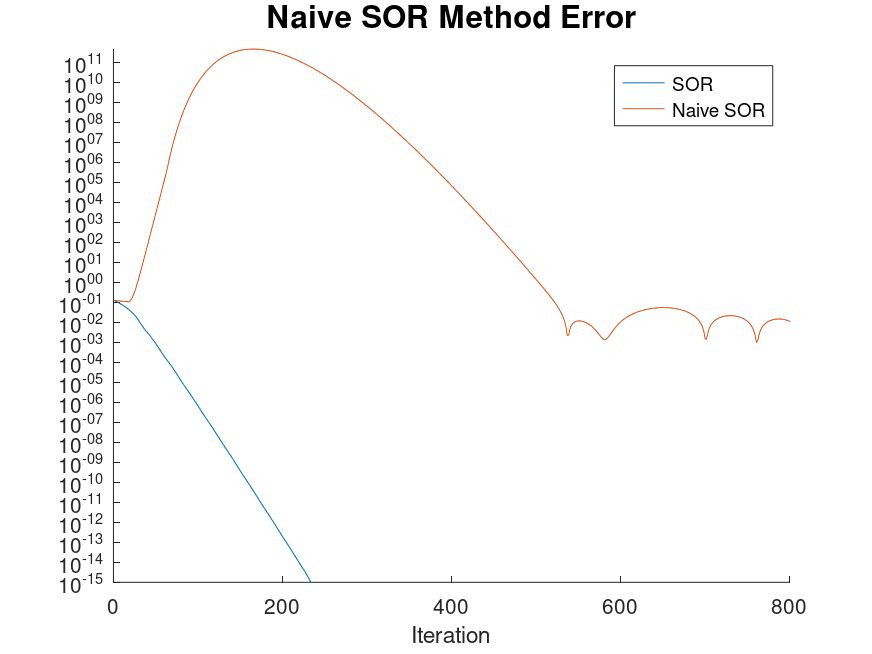
\includegraphics[width=0.7\textwidth]{problem_1d_naive_sor_matrix_splitting_error_800_iterations.png}
        \caption{Comparison of Naive SOR implementation and Correct SOR implementation}
    \end{figure}

    \ \\
\end{solution}